
\documentclass[xcolor=dvipsnames]{beamer}
\usecolortheme[named=OliveGreen]{structure}
\setbeamertemplate{items}[ball]
\setbeamertemplate{blocks}[rounded][shadow=true]
\setbeamertemplate{navigation symbols}{}
\usepackage{graphicx}
\usepackage{amssymb}
\usepackage{tikz}
\usepackage{graphicx}
\usepackage{amsmath}
\usepackage{amsthm}
\usepackage{amssymb}
\usepackage{url}
\usepackage{multirow}
\usepackage{times}
\usepackage{wrapfig}

\usetikzlibrary{backgrounds}
\usetikzlibrary{shapes}
\usetikzlibrary{arrows}


\mode<presentation>
{
  \usetheme{Warsaw}
  % or ...

  \setbeamercovered{transparent}
  % or whatever (possibly just delete it)
}


\usepackage[english]{babel}
% or whatever

\usepackage[utf8]{inputenc}
% or whatever

\usepackage{times}
\usepackage[T1]{fontenc}
% Or whatever. Note that the encoding and the font should match. If T1
% does not look nice, try deleting the line with the fontenc.


\title[DVCS] % (optional, use only with long paper titles)
{Distributed Version Control System}

\subtitle
{}

\author[Rahul,Satvik] % (optional, use only with lots of authors)
{~Rahul Ajmera \\
~Satvik Chauhan}

% - Give the names in the same order as the appear in the paper.
% - Use the \inst{?} command only if the authors have different
%   affiliation.
%\date[CS685] % (optional, should be abbreviation of conference name)
%{CS685}
% - Either use conference name or its abbreviation.
% - Not really informative to the audience, more for people (including
%   yourself) who are reading the slides online

\institute[IITK] % (optional, but mostly needed)
{
  %
  Department of Computer Science and Engineering\\
  Indian Institute of Technology , Kanpur
}
% - Use the \inst command only if there are several affiliations.
% - Keep it simple, no one is interested in your street address.


\subject{DVCS}
% This is only inserted into the PDF information catalog. Can be left
% out.



% If you have a file called "university-logo-filename.xxx", where xxx
% is a graphic format that can be processed by latex or pdflatex,
% resp., then you can add a logo as follows:

 \pgfdeclareimage[height=1.0cm]{university-logo}{university-logo-filename}
 \logo{\pgfuseimage{university-logo}}



% Delete this, if you do not want the table of contents to pop up at
% the beginning of each subsection:
%\AtBeginSubsection[]
%{
%  \begin{frame}<beamer>{Outline}
%    \tableofcontents[currentsection,currentsubsection]
%  \end{frame}
%}


% If you wish to uncover everything in a step-wise fashion, uncomment
% the following command:

%\beamerdefaultoverlayspecification{<+->}


\begin{document}

\begin{frame}
  \titlepage
\end{frame}

\begin{frame}{Outline}
  \tableofcontents
  % You might wish to add the option [pausesections]
\end{frame}


% Structuring a talk is a difficult task and the following structure
% may not be suitable. Here are some rules that apply for this
% solution:

% - Exactly two or three sections (other than the summary).
% - At *most* three subsections per section.
% - Talk about 30s to 2min per frame. So there should be between about
%   15 and 30 frames, all told.

% - A conference audience is likely to know very little of what you
%   are going to talk about. So *simplify*!
% - In a 20min talk, getting the main ideas across is hard
%   enough. Leave out details, even if it means being less precise than
%   you think necessary.
% - If you omit details that are vital to the proof/implementation,
%   just say so once. Everybody will be happy with that.

\section {Introduction}
\subsection{Motivation}

\begin{frame}{Directory history of a person not using Version Control}
\begin{figure}
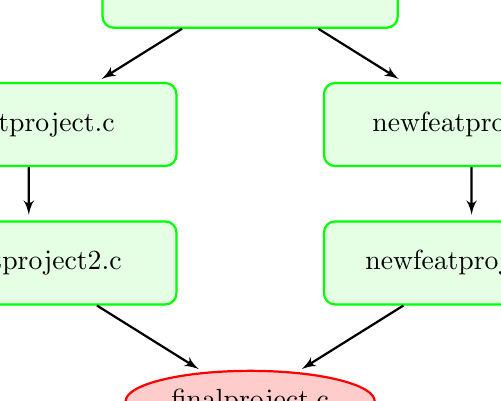
\begin{tikzpicture}[thick,scale=0.8, every node/.style={transform canvas},ampersand replacement=\&]
%\begin{tikzpicture}[auto]
\tikzstyle{decision} = [diamond, draw=blue, thick, fill=blue!20,text badly centered, inner sep=4]
\tikzstyle{block} = [rectangle, draw=green, thick, fill=green!10,
text width=100, text centered, rounded corners, minimum height=30]
\tikzstyle{line} = [draw, thick, -latex',shorten >=2];
\tikzstyle{cloud} = [draw=red, thick, ellipse,fill=red!20, minimum height=20];
\matrix [column sep=80,row sep=50]
{
% row 1
\& \node [block] (p1) {project.c}; \\
\node [block] (p2) {latestproject.c};  \& \& ;
\node [block] (p3) {newfeatproject.c}; \\
\node [block] (p4) {latestproject2.c};  \& \& ;
\node [block] (p5) {newfeatproject2.c}; \\
\& \node [cloud] (p6) {finalproject.c} ;\\
};
\tikzstyle{every path}=[line]
\path  (p1) -- (p2);
\path (p1) -- (p3);
\path (p2) -- (p4);
\path (p3) -- (p5);
\path (p4) -- (p6);
\path (p5) -- (p6);
\end{tikzpicture}
\end{figure}
\end{frame}

\begin{frame}{Motivation}
\begin{itemize}
\item Keep track of changes you made.
\item Revert changes to earlier versions.
\item Share them with collaborators.
\item Work on multiple features simultaneously.
\item Merge two different versions of the files.
\end{itemize}
\end {frame}

\section{Distributed Version Control Systems}
\begin{frame}{Centralized Vs Distributed}

\begin{columns}[c]
\column{5cm}
\framebox{\includegraphics[width=5cm]{cvcs}}
\column{5cm}
\framebox{\includegraphics[width=5cm]{dvcs}}

\end{columns}
\end{frame}

\section{Algorithm}

\subsection{Directory Structure}

\begin{frame}{Changeset Choices}
\begin{itemize}
\item Keep some snapshot versions and incremental diffs from these versions.
\item Keep each commit as separate snapshot.
\item Pros and Cons for each way.
\end{itemize}
\end{frame}

\begin{frame}{Changeset Choices}
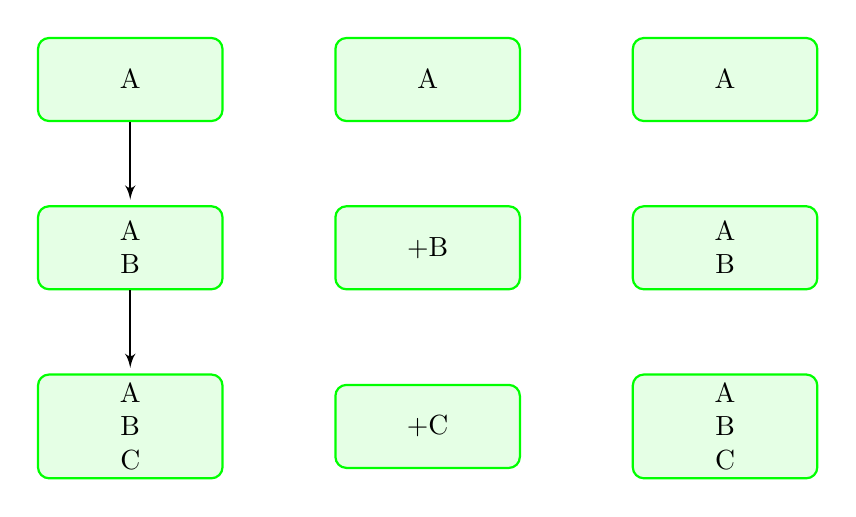
\begin{tikzpicture}[thick,ampersand replacement=\&]
\tikzstyle{decision} = [diamond, draw=blue, thick, fill=blue!20,text badly centered, inner sep=4]
\tikzstyle{block} = [rectangle, draw=green, thick, fill=green!10,
text width=60, text centered, rounded corners, minimum height=30]
\tikzstyle{line} = [draw, thick, -latex',shorten >=2];
\tikzstyle{cloud} = [draw=red, thick, ellipse,fill=red!20, minimum height=20, text width = 20,text centered];
\matrix [column sep=40,row sep=30]
{
% row 1
\node [block] (a1) {A}; \&
\node [block] (b1) {A}; \&
\node [block] (c1) {A };\\
\node [block] (a2) {A \\ B}; \&
\node [block] (b2) {+B}; \&
\node [block] (c2) {A \\  B};\\
\node [block] (a3) {A \\ B \\ C} ; \&
\node [block] (b3) {+C}; \&
\node [block] (c3) {A \\ B \\ C};\\
};
\tikzstyle{every path}=[line]
\path (a1) -- (a2);
\path (a2) -- (a3);
\end{tikzpicture}
\begin{itemize}
\item KISS principle.
\item Modified II version + aggressive compression strategies.
\end{itemize}
\end{frame}

\begin{frame}{Advantages}
\begin{itemize}
\item It is seen that few files are modified with lots of changes between two
  commit.
\item Use hash of files as their filename while taking snapshot.
\item Unchanged files between two commits are not copied.
\item Advantages
\begin{enumerate}
\item Easy Rollbacks.
\item Corruption of one file don't effect its other versions.
\item Aggressive text compression Algorithms can be used to further compress
  the space.
\end{enumerate}
\end {itemize}
\end{frame}

\subsection{Transfer of commits}
\begin{frame}{Sending Commits}
\begin{itemize}
\item Minimize number of communications between peers.
\item Only 3 messages required at the time of pull.
\begin{enumerate}
\item Commits to fetch.
\item Commits compressed and sent.
\end{enumerate}
\item 3-Way merge startegy to merge the files.
\end{itemize}
\end{frame}

\subsection{Structure}
\begin{frame}{Sending Commits}
\begin{figure}
\centering
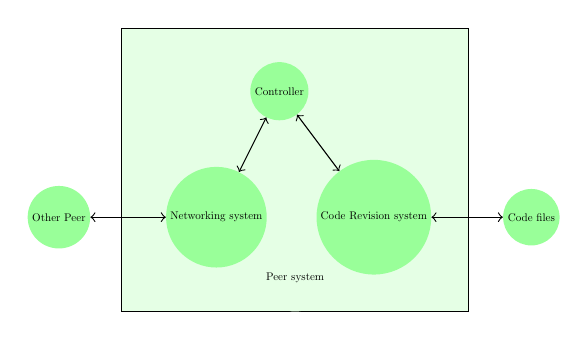
\begin{tikzpicture}[ scale=0.4,transform shape]
\tikzstyle{every node}=[circle,fill=green!40]
\draw [fill=green!10] (-3,-3) rectangle (8,6);
\draw (2.5,-3) node [above ,fill=green!10] {Peer system};
\node (a) at (0,0) {Networking system} ;
\node (b) at (5,0) {Code Revision system};
\node (c) at (2,4) {Controller};
\node (f) at (10,0) {Code files};
\node (u) at (-5,0) {Other Peer};
\draw [<->] (c) -- (a);
\draw [<->] (c) -- (b);
\draw [<->] (u) -- (a);
\draw [<->] (b) -- (f);
\end{tikzpicture}
\caption{Highlevel design}
\end{figure}
\begin{itemize}
\item Command line UI.
\item Graphical User Interface (Not very flexible).
\end{itemize}
\end{frame}

\section{Conclusion and Future work}
\begin{frame}{Conclusion and Future work}
\begin{itemize}
\item Covers basic features of distributed version control system.
\item Enhancements
\begin{enumerate}
\item Branch support.
\item Automatic fetching of commits from added hosts.
\item More flexible GUI and command line UI.
\end{enumerate}
\end{itemize}


\end{frame}

\end{document}
